\section{Постановка задачи и описание данных}
\label{sec:Chapter1}

\subsection{Формальная постановка задачи}

Пусть задана выборка $\mathcal{D} = \{(\mathbf{x}_i,\, y_i)\}_{i=1}^{N}$,
где $\mathbf{x}_i \in \mathbb{R}^d$~--- вектор признаков $i$-го кардиоцикла,
$y_i \in \mathcal{Y} = \{\text{N},\,\text{A},\,\text{V},\,\text{L},\,\text{R}\}$~---
его класс, $N = 100\,025$~--- общее число объектов, $d = 240$~--- размерность
пространства признаков.

\textbf{Задача классификации.}
Требуется построить функцию $f\colon \mathbb{R}^d \to \mathcal{Y}$,
минимизирующую макроусредненную ошибку классификации по всем классам:
\begin{equation}
    \label{eq:macro_f1}
    \text{Macro\,F1} = \frac{1}{|\mathcal{Y}|}\sum_{k \in \mathcal{Y}}
    \frac{2\,\mathrm{TP}_k}{2\,\mathrm{TP}_k + \mathrm{FP}_k + \mathrm{FN}_k}\,,
\end{equation}
где $\mathrm{TP}_k$, $\mathrm{FP}_k$, $\mathrm{FN}_k$~---
число истинно положительных, ложно положительных и~ложно отрицательных
срабатываний модели для класса~$k$ соответственно.

Метрика Macro~F1 выбрана основной, поскольку она одинаково взвешивает все
классы независимо от~их частоты в~выборке~--- что~принципиально важно при
сильном дисбалансе (класс~A составляет лишь $2.5\,\%$ выборки).
Дополнительно отслеживаются Accuracy и Weighted~F1.

\subsection{Описание данных}

\subsubsection{База данных MIT-BIH Arrhythmia Database}

В~работе используется открытая база MIT-BIH Arrhythmia
Database~\cite{moody2001,physionet2000}~--- международный стандарт для
оценки алгоритмов обнаружения аритмий~\cite{aami2012}.
База содержит $48$ двухканальных записей ЭКГ по $30$~минут каждая,
оцифрованных с~частотой дискретизации $f_s = 360$~Гц при разрядности
$11$~бит ($\pm 5$~мВ в диапазоне).
Каждое сердечное сокращение размечено двумя независимыми
кардиологами-экспертами.

\subsubsection{Классы аритмий}

Из~полного набора символов аннотаций выбраны $5$ клинически значимых
классов, охватывающих наиболее распространенные нарушения ритма
(таблица~\ref{tab:class_dist}).

\begin{table}[h]
\centering
\caption{Распределение классов в итоговой выборке}
\label{tab:class_dist}
\begin{tabular}{clrrc}
\hline
\textbf{Символ} & \textbf{Клиническое название} & \textbf{Число ударов} &
\textbf{Доля, \%} & \textbf{Отношение к~N} \\
\hline
N & Норма                               & 75\,023 & 75.0 & $1\!:\!1$    \\
L & Блокада левой ножки пучка Гиса      &  8\,075 &  8.1 & $1\!:\!9.3$  \\
R & Блокада правой ножки пучка Гиса     &  7\,259 &  7.3 & $1\!:\!10.3$ \\
V & Желудочковая экстрасистола           &  7\,129 &  7.1 & $1\!:\!10.5$ \\
A & Предсердная экстрасистола            &  2\,539 &  2.5 & $1\!:\!29.6$ \\
\hline
  & \textbf{Итого}                      & \textbf{100\,025} &
  \textbf{100} & --- \\
\hline
\end{tabular}
\end{table}

Класс~N существенно преобладает~--- соотношение «норма\,:\,предсердная
экстрасистола» составляет~$\approx 30\!:\!1$.
Такой дисбаланс классов является типичной проблемой медицинских
данных и~требует специальных мер как~при~обучении моделей,
так~и~при~выборе метрики качества.

\subsubsection{Предобработка: извлечение кардиоциклов}

Каждый кардиоцикл вырезается из~записи в~виде окна фиксированного
размера $d = 240$ отсчетов с~центром в~R-пике~--- точке максимальной
амплитуды комплекса QRS (рисунок~\ref{fig:beat_window}):
\begin{equation}
    \label{eq:window}
    \mathbf{x}_i = \bigl(s[r_i - 100],\; s[r_i - 99],\; \ldots,\;
    s[r_i + 139]\bigr) \in \mathbb{R}^{240},
\end{equation}
где $s[\cdot]$~--- отсчеты сигнала ЭКГ, $r_i$~--- позиция R-пика
$i$-го удара из~аннотации базы данных.
Выбор асимметричного окна $100 + 140$ обусловлен тем, что~зубец~P
расположен непосредственно перед~QRS, тогда как~зубец~T после
него~--- более протяженный.
При~$f_s = 360$~Гц окно длиной~$240$ отсчетов соответствует
$\approx 667$~мс, что~достаточно для~фиксации полного кардиоцикла
при~частоте пульса до~$\approx 90$~уд/мин.
Удары, для~которых окно выходит за~границы записи, исключаются.

\begin{figure}[h]
\centering
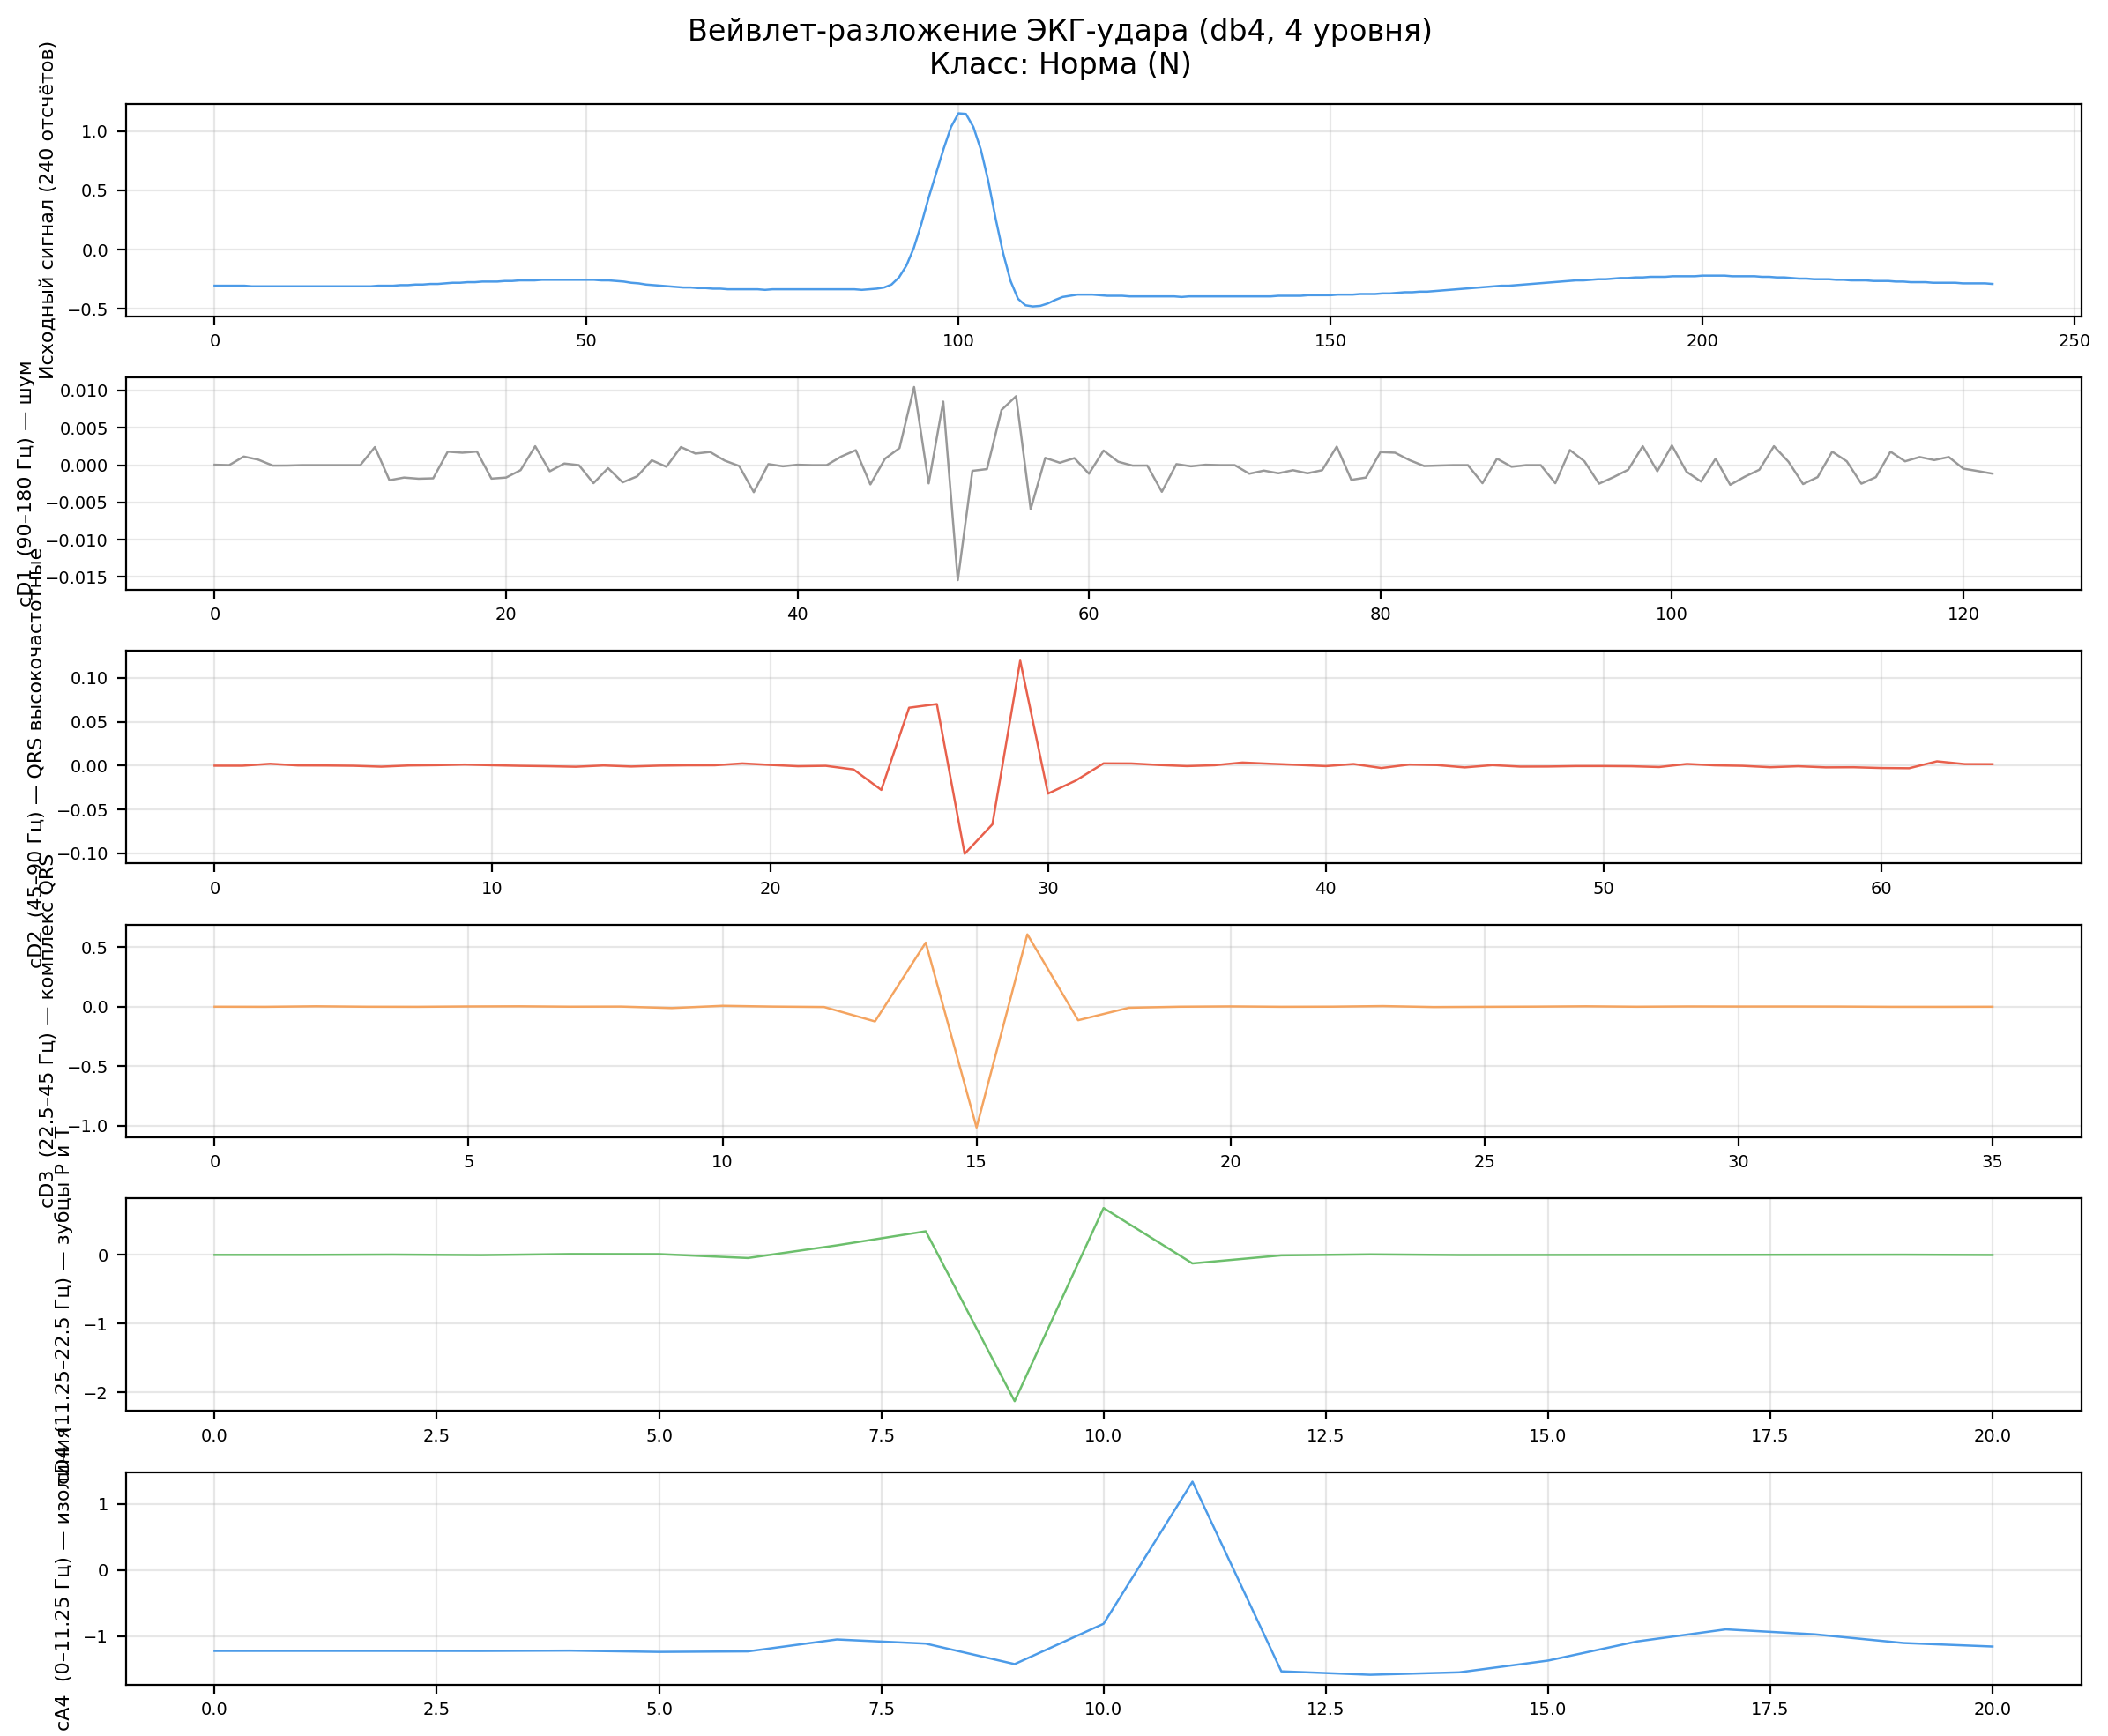
\includegraphics[width=0.85\textwidth]{../reports/figures/models/wavelet_decomposition_N.png}
\caption{Вейвлет-разложение нормального кардиоцикла (класс~N):
исходный сигнал и уровни ДВП db4.
По оси абсцисс~--- номер отсчета; по оси ординат~--- амплитуда в~мВ.}
\label{fig:beat_window}
\end{figure}

\subsubsection{Нормализация}

Для~нейронных сетей каждый признак нормализуется по~обучающей выборке
с~помощью стандартного масштабирования:
\begin{equation}
    \label{eq:scaler}
    \tilde{x}_{ij} = \frac{x_{ij} - \hat{\mu}_j}{\hat{\sigma}_j}\,,
    \quad j = 1, \ldots, d,
\end{equation}
где $\hat{\mu}_j$ и~$\hat{\sigma}_j$~--- выборочные среднее и~стандартное
отклонение $j$-го признака по~обучающей выборке.
Параметры нормализации вычисляются исключительно на~обучающих данных
и~применяются к~тестовой выборке без повторной подгонки~---
во~избежание «утечки» информации из~теста.
Для~случайного леса нормализация не~требуется, поскольку деревья
решений инвариантны к~монотонным преобразованиям признаков.

\subsection{Разбиение на выборки}

Выборка разбивается на~обучающую $(80\,\%)$ и~тестовую $(20\,\%)$
части методом стратифицированного разбиения:
\begin{equation}
    |\mathcal{D}_\text{train}| = 80\,020, \quad
    |\mathcal{D}_\text{test}| = 20\,005.
\end{equation}
Стратификация гарантирует, что~доля каждого класса в~обеих частях
совпадает с~долей в~исходной выборке.
Фиксированный начальный номер генератора случайных чисел
(\texttt{random\_state=42}) обеспечивает воспроизводимость результатов.

Для~оценки стабильности моделей дополнительно проводится
пятикратная стратифицированная кросс-валидация~(см.~раздел~\ref{sec:Chapter4}).

\subsection{Проблема дисбаланса классов и способы ее решения}

Сильный дисбаланс классов~--- в~первую очередь малочисленность
класса~A~--- порождает систематическое смещение модели в~пользу
большинства: модель, предсказывающая «норму» для~всех объектов,
достигает Accuracy~$\approx 75\,\%$, оставаясь при~этом клинически
бесполезной.

В~данной работе применяются два независимых механизма компенсации
дисбаланса:

\begin{enumerate}
    \item \textbf{Взвешенная функция потерь} для~нейронных сетей.
    Каждому классу~$k$ назначается вес, обратно пропорциональный
    его частоте в~обучающей выборке:
    \begin{equation}
        \label{eq:weights}
        w_k = \frac{1/n_k}{\sum_{j \in \mathcal{Y}} 1/n_j}
        \cdot |\mathcal{Y}|,
    \end{equation}
    где $n_k$~--- число объектов класса~$k$ в~обучающей части.
    Взвешенная кросс-энтропия:
    \begin{equation}
        \label{eq:wce}
        \mathcal{L} = -\sum_{k \in \mathcal{Y}} w_k \sum_{i:\,y_i=k}
        \log \hat{p}_{ik},
    \end{equation}
    где $\hat{p}_{ik}$~--- предсказанная вероятность класса~$k$
    для~объекта~$i$.

    \item \textbf{Стратегия \texttt{balanced\_subsample}} для~случайного
    леса: при~построении каждого дерева обучающая выборка
    для~бутстрэпа ресамплируется с~равномерным представлением
    всех классов.
\end{enumerate}

\subsection{Требования к решению}

По~итогам работы решение должно удовлетворять следующим требованиям:

\begin{itemize}
    \item Macro~F1 не~ниже $0.90$ на~тестовой выборке для каждой
          из~трех моделей.
    \item Recall класса~A (предсердная экстрасистола) не~ниже $0.65$~---
          клинически значимое нарушение не~должно систематически
          пропускаться.
    \item Стандартное отклонение Macro~F1 по~фолдам кросс-валидации
          не~выше~$0.03$~--- требование к~стабильности модели.
    \item Модели должны быть сохранены в~воспроизводимом формате
          для~последующего применения на~новых записях.
\end{itemize}
